\documentclass{article}
\usepackage[landscape]{geometry}
\usepackage{url}
\usepackage{multicol}
\usepackage{amsmath}
\usepackage{esint}
\usepackage{amsfonts}
\usepackage{tikz}
\usetikzlibrary{decorations.pathmorphing}
\usepackage{amsmath,amssymb}
\usepackage{graphicx}
\usepackage{float}
\usepackage{colortbl}
\usepackage{xcolor}
\usepackage{mathtools}
\usepackage{amsmath,amssymb}
\usepackage{enumitem}
\usepackage[symbol]{footmisc}
\makeatletter

\newcommand*\bigcdot{\mathpalette\bigcdot@{.5}}
\newcommand*\bigcdot@[2]{\mathbin{\vcenter{\hbox{\scalebox{#2}{$\m@th#1\bullet$}}}}}
\renewcommand{\thempfootnote}{\fnsymbol{mpfootnote}}
\makeatother

\title{Unit 1 Summary Sheet}
\usepackage[T1]{fontenc}
\usepackage[utf8]{inputenc}
\usepackage[english]{babel}

\advance\topmargin-.8in
\advance\textheight3in
\advance\textwidth3in
\advance\oddsidemargin-1.5in
\advance\evensidemargin-1.5in
\parindent0pt
\parskip2pt
\newcommand{\hr}{\centerline{\rule{3.5in}{1pt}}}
%\colorbox[HTML]{e4e4e4}{\makebox[\textwidth-2\fboxsep][l]{texto}
\begin{document}

\begin{center}{\huge{\textbf{Unit 3 Summary Sheet}}}\\
\end{center}
\begin{multicols*}{3}

\tikzstyle{mybox} = [draw=black, fill=white, very thick,
    rectangle, rounded corners, inner sep=10pt, inner ysep=10pt]
\tikzstyle{fancytitle} =[fill=black, text=white, font=\bfseries]

%------------ Kinetic Molecular Theory ---------------
\begin{tikzpicture}
\node [mybox] (box){%
    \begin{minipage}{0.3\textwidth}
    \textbf{States of Matter}: solid, liquid, or gas. \\
    \textbf{Solid}: has small spaces between particles, and slow motion of particles. \\ \\
    \small{
    	\begin{tabular}{ | c | c | }
        \hline
	Description & - ordered and dense \\
	& - has a definite shape and volume \\
	& - virtually incompressible \\
	\hline
	\end{tabular}} \\ \\
    \textbf{Liquid}: has medium spaces between particles, and medium motion of particles. \\ \\
    \small{
    	\begin{tabular}{ | c | c | }
        \hline
	Description & - disordered and low density \\
	& - has definite volume \\
	& - takes the shape of the container \\
	& - slightly compressible \\
	\hline
	\end{tabular}} \\ \\
    \textbf{Gas}: has large spaces between particles, and fast motion of particles. \\ \\
    \small{
    	\begin{tabular}{ | c | c | }
        \hline
	Description & - disordered and very low density \\
	& - does not have a definite shape \\
	& - does not have a definite volume \\
	& - highly incompressible \\
	\hline
	\end{tabular}} \\ \\
    \textbf{Types of Motion}: vibrational, rotational, or translational. \\
    \textbf{Vibrational}: has a back and forth motion; occurs in solids, liquids and gases. \\
    \textbf{Rotational}: has a spinning motion; occurs in liquids and gases. \\
    \textbf{Translational}: movement is in a straight line; occurs in liquids and gases. \\ \\
    \textbf{Kinetic Molecular Theory}: states that gas particles behave like hard, spherical objects that are in constant, random motion. \\
    \textbf{Temperature}: is a measure of the average kinetic energy of entities in a sample. \\
    \textbf{Kinetic Energy}: form of energy that an object or particles has. The average kinetic energy of gas particles is directly proportional to the absolute temperature. \\ \\
    $T\propto {KE}_{avg}$ \\
    \begin{itemize}
        \item $\uparrow$ absolute temperature = $\uparrow$ motion of gas particles
        \item $\uparrow$ motion of gas particles = $\uparrow$ average KE
    \end{itemize}
    \textit{At a given temperature, all gas entities have the same average kinetic energy regardless of their size or mass.}
    \end{minipage}
};
%------------ Kinetic Molecular Theory Header ---------------------
\node[fancytitle, right=10pt] at (box.north west) {Kinetic Molecular Theory};
\end{tikzpicture}

%------------ Atmospheric Pressure ---------------
\begin{tikzpicture}
\node [mybox] (box){%
    \begin{minipage}{0.3\textwidth}
    \textbf{Atmospheric Pressure}: the amount of force per unit area exerted by air on all objects. \\
    $\displaystyle{P=\frac{F}{A}}$
    \begin{itemize}
        \item $\uparrow$ force = $\uparrow$ pressure, $F\propto P$
	\item $\uparrow$ area = $\downarrow$ pressure, $\displaystyle{A\propto\frac{1}{P}}$
	\item pressure is a physical property of gas.
	\item collisions of gas particles occur, pressure is caused when gas particles hit the walls of their container.
    \end{itemize}
    \textbf{Pascal}: SI unit for pressure.
    \begin{itemize}
        \item $\displaystyle{Pa=\frac{N}{m^{2}}=\frac{kg}{m\times s^{2}}}$
        \item kilopascal is often used, $kPa=1000\,Pa$
    \end{itemize}
    \textbf{Absolute Temperature}: is temperature measured using the Kelvin scale where zero is absolute zero.
    \begin{itemize}
        \item $0\,K=-273.15^{\circ}C$
        \item $T_{K}=T_{^{\circ}C}+273.15$
        \item $T_{^{\circ}C}=T_{K}-273.15$
    \end{itemize}
    \textbf{Standard Atmosphere}: 1 atm is approximately Earth's atmospheric pressure at sea level. \\
    \textbf{Standard Temperature and Pressure (STP)}
    \begin{itemize}
        \item temperature = $0^{\circ}C$ = 273.15 K
	\item pressure = 1 atm = 101.325 kPa = 760 mmHg = 760 torr
	\item volume = 22.4 L/mol
    \end{itemize}
    \textbf{Standard Ambient Temperature and Pressure (SATP)}
    \begin{itemize}
	\item temperature = $25^{\circ}$ = 298.15 K
	\item pressure = 100 kPa
	\item volume = 24.8 L/mol
    \end{itemize}
    \end{minipage}
};
%------------ Atmospheric Pressure Header ---------------------
\node[fancytitle, right=10pt] at (box.north west) {Atmospheric Pressure};
\end{tikzpicture}

%------------ Charles' Law ---------------
\begin{tikzpicture}
\node [mybox] (box){%
    \begin{minipage}{0.3\textwidth}
    \textbf{Volume and Temperature}: French scientist Jacques Charles (1746-1823) examined the expansion of a variety of gases. \\
    \textbf{Charles' Law}: the volume of an ideal gas is directly proportional to the absolute temperature, provided the pressure and the amount of gas remain constant. \\ \\
    $\displaystyle{\frac{V_{1}}{T_{1}}=\frac{V_{2}}{T_{2}}}$, or $\displaystyle{\frac{V}{T}=a}$ (constant)
    \begin{itemize}
        \item Since $\displaystyle{V\propto T}$, then $\displaystyle{V=aT}$ (a is a constant).
        \item $\uparrow$ volume = $\uparrow$ absolute temperature.
        \item temperature must be in kelvin.
    \end{itemize}
    \textbf{Kelvin Scale}: a scale of temperature in which absolute zero is zero (0 K).
    \begin{itemize}
        \item determined that at absolute zero (0 K) the particles in a substance are motionless.
        \item kinetic energy would be zero.
	\item theoretically, the volume of gas would be zero.
    \end{itemize}
    \begin{figure}[H]
	\centering
	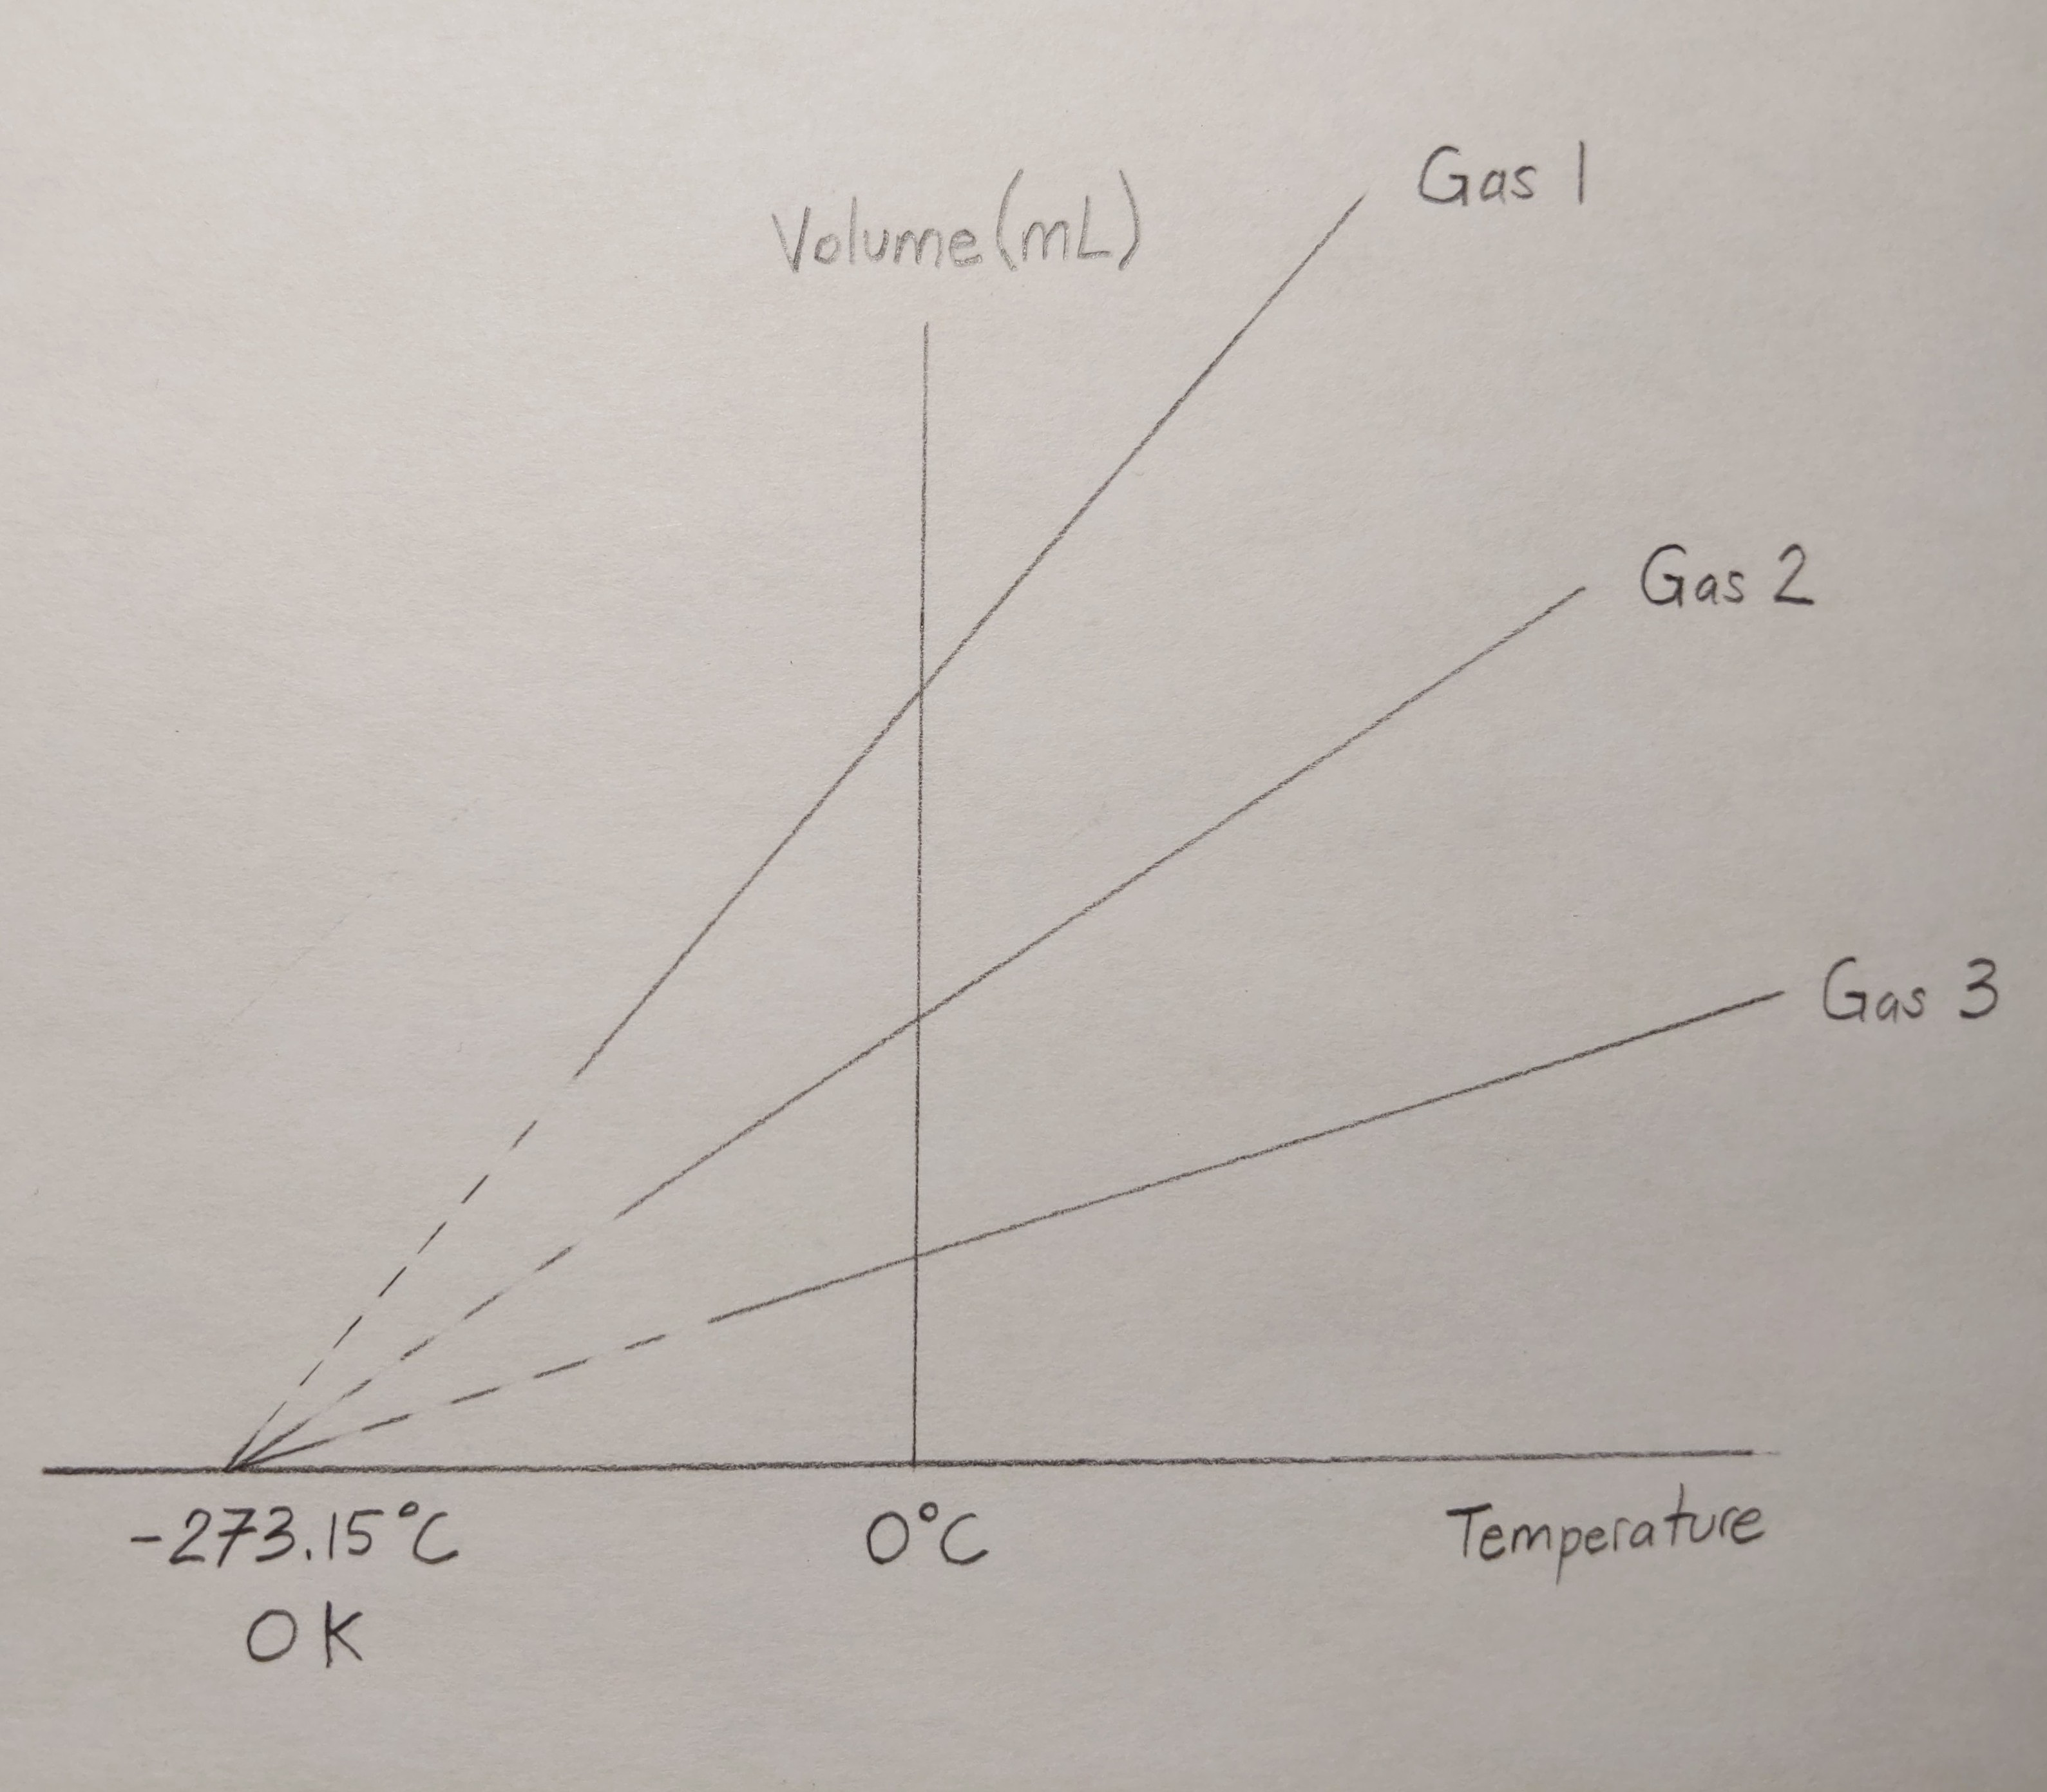
\includegraphics[scale=0.07]{diagrams/charles-law.jpg}
        \caption{Charles' Law Graph\protect\footnote[2]{Dashed lines are extrapolated, lines meet at absolute zero.}}
        \label{fig:charles}
    \end{figure}
    \end{minipage}
};
%------------ Charles' Law Header ---------------------
\node[fancytitle, right=10pt] at (box.north west) {Charles' Law};
\end{tikzpicture}

%------------ Boyle's Law ---------------
\begin{tikzpicture}
\node [mybox] (box){%
    \begin{minipage}{0.3\textwidth}
    \textbf{Volume and Pressure}: Anglo-Irish chemist Robert Boyle (1627-1691) examined how the volume of a gas decreases with increasing pressure and vise versa. \\
    \textbf{Boyle's Law}: The volume of a gas is inversely proportional to its pressure, provided the temperature and the amount of gas remain constant. \\ \\
    $\displaystyle{P_{1}V_{1}=P_{2}V_{2}}$, or $PV=k$ (k is a constant)
    \begin{itemize}
        \item Since $\displaystyle{V\propto\frac{1}{P}}$, then $\displaystyle{V=\frac{k}{P}}$ (k is a constant).
        \item as volume $\uparrow$, then pressure $\downarrow$.
        \item as volume $\downarrow$, then pressure $\uparrow$.
    \end{itemize}
    \end{minipage}
};
%------------ Boyle's Law Header ---------------------
\node[fancytitle, right=10pt] at (box.north west) {Boyle's Law};
\end{tikzpicture}

%------------ Gay-Lussac's Law ---------------
\begin{tikzpicture}
\node [mybox] (box){%
    \begin{minipage}{0.3\textwidth}
    \textbf{Pressure and Temperature}: French chemist Gay-Lussac (1778-1850) examined how the pressure of a gas increases proportionally as its temperature increases and vise versa. \\
    \textbf{Gay-Lussac's Law}: The pressure of a gas is directly proportional to its temperature, provided the volume and the amount of gas remain constant. \\ \\
    $\displaystyle{\frac{P_{1}}{T_{1}}=\frac{P_{2}}{T_{2}}}$, or $\displaystyle{\frac{P}{T}=k}$ (k is a constant)
    \begin{itemize}
        \item Since $\displaystyle{P\propto T}$, then $\displaystyle{P=kT}$ (k is a constant).
        \item as absolute temperature $\uparrow$, then pressure $\uparrow$.
        \item temperature must be in kelvin.
    \end{itemize}
    \end{minipage}
};
%------------ Gay-Lussac's Law Header ---------------------
\node[fancytitle, right=10pt] at (box.north west) {Gay-Lussac's Law};
\end{tikzpicture}

%------------ Combined Gas Law ---------------
\begin{tikzpicture}
\node [mybox] (box){%
    \begin{minipage}{0.3\textwidth}
    The \textbf{combined gas law} describes the relationship between volume, temperature, and pressure for any fixed amount of gas. \\
    The \textbf{Combined Gas Law}: The product of the pressure and volume of a gas divided by its absolute temperature is a constant, provided the amount of gas is kept constant. \\ \\
    $\displaystyle{\frac{P_{1}V_{1}}{T_{1}}=\frac{P_{2}V_{2}}{T_{2}}}$, or $\displaystyle{\frac{PV}{T}=constant}$
    \begin{itemize}
        \item amount of gas remains constant.
        \item temperature must be in kelvin.
    \end{itemize}
    \end{minipage}
};
%------------ Combined Gas Law Header ---------------------
\node[fancytitle, right=10pt] at (box.north west) {Combined Gas Law};
\end{tikzpicture}

%------------ Law of Combining Volumes ---------------
\begin{tikzpicture}
\node [mybox] (box){%
    \begin{minipage}{0.3\textwidth}
    Gay-Lussac proposed the \textbf{law of combining gases} during when the kinetic molecular theory had not yet been developed. \\
    Amedeo Avogadro later on proposes the explanation for the law of combining volumes. \\
    \textbf{Law of Combining Volumes}: gases always react to produce products in whole-number ratios when measured at the same temperature and pressure. \\
    \textbf{Volume Ratios}: are the same as the coefficients in a balanced chemical equation.
    \end{minipage}
};
%------------ Law of Combining Volumes Header ---------------------
\node[fancytitle, right=10pt] at (box.north west) {Law of Combining Volumes};
\end{tikzpicture}

%------------ Avogadro's Law ---------------
\begin{tikzpicture}
\node [mybox] (box){%
    \begin{minipage}{0.3\textwidth}
    \textbf{Volume and Amount of Gas}: Italian scientist Amedeo Avogadro (1776-1856) discovered that equal volumes of gases, at the same temperature and pressure, contain the same number of molecules. \\
    \textbf{Avogadro's Law}: The volume of a gas is directly proportional to the amount of gas, provided the temperature and pressure remain constant. \\ \\
    $\displaystyle{\frac{V_{1}}{n_{1}}=\frac{V_{2}}{n_{2}}}$, or $\displaystyle{\frac{V}{n}=constant}$
    \begin{itemize}
        \item Since $\displaystyle{V\propto n}$, then $\displaystyle{V=kn}$ (k is a constant).
        \item equal volumes of gas at the same temperature and pressure contain an equal number of molecules.
        \item this explains why the mole ratios in a balanced chemical equation are also the ratios of volumes.
    \end{itemize}
    \end{minipage}
};
%------------ Avogadro's Law Header ---------------------
\node[fancytitle, right=10pt] at (box.north west) {Avogadro's Law};
\end{tikzpicture}

%------------ Molar Volume ---------------
\begin{tikzpicture}
\node [mybox] (box){%
    \begin{minipage}{0.3\textwidth}
    \textbf{Molar Volume}: is the volume occupied by one mole of gas at a specified temperature and pressure.
    \begin{itemize}
        \item At STP, one mole of any gas occupies 22.4 L.
        \item At SATP, one mole of any gas occupies 24.8 L.
    \end{itemize}
    \end{minipage}
};
%------------ Molar Volume Header ---------------------
\node[fancytitle, right=10pt] at (box.north west) {Molar Volume};
\end{tikzpicture}

%------------ Gas Density ---------------
\begin{tikzpicture}
\node [mybox] (box){%
    \begin{minipage}{0.3\textwidth}
    $${density=\frac{mass}{volume}}$$
    \begin{itemize}
        \item for mass, use the molar mass (g/mol).
        \item for volume, use the molar volume (L/mol).
    \end{itemize}
    \end{minipage}
};
%------------ Gas Density Header ---------------------
\node[fancytitle, right=10pt] at (box.north west) {Gas Density};
\end{tikzpicture}

%------------ Ideal Gases ---------------
\begin{tikzpicture}
\node [mybox] (box){%
    \begin{minipage}{0.3\textwidth}
    An \textbf{ideal gas} has the following properties:
    \begin{itemize}
        \item all entities of an ideal gas have high translational energy, moving randomly in all directions (in straight lines).
        \item collision of ideal gas entities with each other or with the wall of a container are perfectly elastic.
	\item the volume of an ideal gas entity is negligible (zero) compared to the volume of a container.
	\item there are no attractive or repulsive forces between ideal gas entities.
	\item ideal gases do not condense into liquid when cooled.
    \end{itemize}
    \textit{There is no such thing as an ideal gas}.
    \end{minipage}
};
%------------ Ideal Gases Header ---------------------
\node[fancytitle, right=10pt] at (box.north west) {Ideal Gases};
\end{tikzpicture}

%------------ The Ideal Gas Law ---------------
\begin{tikzpicture}
\node [mybox] (box){%
    \begin{minipage}{0.3\textwidth}
    Combining Charles' Law, Avogadro's Law, and Boyle's Law, we arrive at the \textbf{ideal gas law}: \\ \\
    $PV=nRT$
    \begin{itemize}
        \item universal gas constant $\displaystyle{R=8.314\frac{kPa\times L}{mol\times K}}$
    \end{itemize}
    \end{minipage}
};
%------------ The Ideal Gas Law Header ---------------------
\node[fancytitle, right=10pt] at (box.north west) {The Ideal Gas Law};
\end{tikzpicture}

%------------ Gas Stoichiometry ---------------
\begin{tikzpicture}
\node [mybox] (box){%
    \begin{minipage}{0.3\textwidth}
    Use one or a combination of the following to solve gas stoichiometry problems:
    \begin{enumerate}
        \item Law of Combining Volumes
        \item Avogadro's Law
        \item Ideal Gas Law
    \end{enumerate}
    \end{minipage}
};
%------------ Gas Stoichiometry Header ---------------------
\node[fancytitle, right=10pt] at (box.north west) {Gas Stoichiometry};
\end{tikzpicture}

%------------ Law of Partial Pressures ---------------
\begin{tikzpicture}
\node [mybox] (box){%
    \begin{minipage}{0.3\textwidth}
    \textbf{Dalton's Law of Partial Pressures}: The total pressure of a mixture of non-reacting gases is equal to the sum of the individual gases' partial pressures. \\
    $P_{total}=P_{1}+P_{2}+P_{3}+...$ \\ \\
    The \textbf{partial pressure} of each individual gas: \\
    $P_{1}=P_{total}\times(\%\,of\,gas\,1)$ \\
    $P_{2}=P_{total}\times(\%\,of\,gas\,2)$ \\
    \vdots
    \end{minipage}
};
%------------ Law of Partial Pressures Header ---------------------
\node[fancytitle, right=10pt] at (box.north west) {Law of Partial Pressures};
\end{tikzpicture}

\end{multicols*}
\end{document}
